%%%%%%%%%%%%%%%%%%%%%%%%%%%%%%%%%%%%%%%%%
% Developer CV
% LaTeX Class
% Version 2.0 (12/10/23)
%
% This class originates from:
% http://www.LaTeXTemplates.com
%
% Authors:
% Omar Roldan
% Based on a template by  Jan Vorisek (jan@vorisek.me)
% Based on a template by Jan Küster (info@jankuester.com)
% Modified for LaTeX Templates by Vel (vel@LaTeXTemplates.com)
%
% License:
% The MIT License (see included LICENSE file)
%
%%%%%%%%%%%%%%%%%%%%%%%%%%%%%%%%%%%%%%%%%

%----------------------------------------------------------------------------------------
%	PACKAGES AND OTHER DOCUMENT CONFIGURATIONS
%----------------------------------------------------------------------------------------

\documentclass[9pt]{developercv} % Default font size, values from 8-12pt are recommended
\usepackage{multicol}
\usepackage{graphicx}
\setlength{\columnsep}{0mm}
%----------------------------------------------------------------------------------------
\usepackage{lipsum}  


\begin{document}

%----------------------------------------------------------------------------------------
%	TITLE AND CONTACT INFORMATION
%----------------------------------------------------------------------------------------
\begin{minipage}[t]{0.2\textwidth} 
	\vspace{-\baselineskip} % Required for vertically aligning minipages

		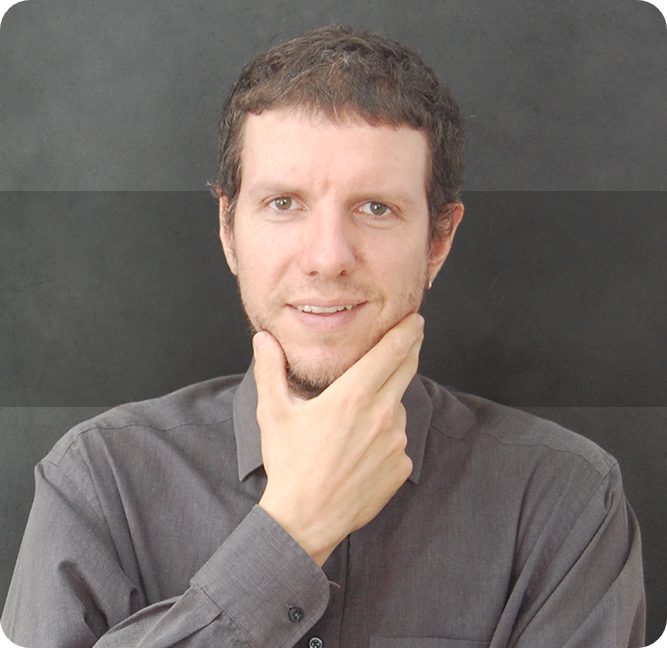
\includegraphics[width=0.7\linewidth]{caio-round.png}
	
\end{minipage}
\begin{minipage}[t]{0.3\textwidth} 
	\vspace{-\baselineskip} % Required for vertically aligning minipages
	
	{ \fontsize{16}{20} \textcolor{black}{\textbf{\MakeUppercase{Caio Laganá \\[1mm]Fernandes}}}} % First name
	
	\vspace{6pt}
	
	{\Large Ph.D Physicist\\[1mm]} % Career or current job title
	Developer
\end{minipage}
\hfill
\begin{minipage}[t]{0.2\textwidth} % 20% of the page width for the first row of icons
	\vspace{-\baselineskip} % Required for vertically aligning minipages
	
	% The first parameter is the FontAwesome icon name, the second is the box size and the third is the text
	\icon{Globe}{11}{\href{http://www.caiolagana.com.br}{caiolagana.com.br}}\\ 
  \icon{Phone}{11}{+55 35 99754 9882}\\
  \icon{MapMarker}{11}{São Paulo, Brazil}\\
	
\end{minipage}
\begin{minipage}[t]{0.27\textwidth} % 27% of the page width for the second row of icons
	\vspace{-\baselineskip} % Required for vertically aligning minipages
	
	\icon{Envelope}{11}{\href{mailto:caiolagana@gmail.com}{caiolagana@gmail.com}}\\	
    \icon{Github}{11}{\href{https://github.com/caiolagana}{github.com/caiolagana}}\\
    \icon{LinkedinSquare}{11}{\href{https://www.linkedin.com/in/caiolagana}{linkedin.com/in/caiolagana}}\\    
    
\end{minipage}


%----------------------------------------------------------------------------------------
%	INTRODUCTION, SKILLS AND TECHNOLOGIES
%----------------------------------------------------------------------------------------

\begin{minipage}[t]{0.46\textwidth}
    \cvsect{Summary}
	\vspace{-6pt}

	Possess Ph.D. in High Energy Nuclear Physics at the European Organization for Nuclear Research (CERN). Awarded the Best Doctorate Thesis Prize by the Brazilian Physical Society in 2020. Experienced in programming languages, software development and data analysis.
\end{minipage}
\hfill % Whitespace between
\begin{minipage}[t]{0.465\textwidth}
    \cvsect{Skills}
    \vspace{-6pt}

	\begin{minipage}[t]{0.35\textwidth}
		\textbf{Portuguese} (native)\vspace{0.5mm}\\
		\textbf{English} (fluent)\vspace{0.5mm}\\
		\textbf{Italian} (fluent)\vspace{0.5mm}\\
		\textbf{French} (functional)\vspace{0.5mm}\\
		\textbf{German} (beginner)
    \end{minipage}
    \hfill
    \begin{minipage}[t]{0.55\textwidth}
	Ability to understand complex systems and work out efficient solutions to intrincate problems
    \end{minipage}
    
\end{minipage}


\vspace{10 pt}
\cvsect{Projects}
\begin{entrylist}
	\entry
		{C++}
		{Hypernuclei Search at CERN}
		{https://github.com/caiolagana/LnnTTreeCreator}
		{This C++ project was written as part of my Ph.D program. It searchs for the $\Lambda nn$ and $\Lambda pn$ hypernuclei in high-energy Pb-Pb collisions at the Large Hadron Collider. The script was ran over thousands of terabytes of data at CERN's computing infrastructure.}
    \entry
		{Visual C\#, SQL}
		{Hydroelectric Power Plant Simulator}
		{https://github.com/caiolagana/PowerPlantSimulator}
		{%Dummy text 
        \lipsum[1][1-3]}
    \entry
		{Python, AngularJS}
		{AI Analysis of Legal Documents}
		{https://github.com/e-fluxus/ia}
		{%Dummy text 
        \lipsum[1][1-3]}
\end{entrylist}



\vspace{-10 pt}
\cvsect{Formal Education}
\begin{entrylist}
    \entry
		{2013 - 2017}
		{Doctorate in Physics}
		{USP/CERN}
		{University of São Paulo (USP) with one-year exchange program at European Organization for Nuclear Research (CERN). {\it Title:} Evidence for the existence of the $\Lambda nn$ hypernucleus with the ALICE detector}
    \entry
		{2010-2012}
		{Master's in Physics}
		{UNESP}
		{State University of São Paulo (UNESP) {\it Title:} Femtoscopia de colisões próton-próton no detector CMS do Large Hadron Collider}
	\entry
		{2006-2010}
		{Bachelor's in Physics}
		{USP}
		{Scholarship from Conselho Nacional de Desenvolvimento Científico e Tecnológico (CNPq)}
\end{entrylist}



\vspace{-10 pt}
\cvsect{Complementary Education}
\begin{entrylist}
    \entry
		{2012}
		{Excellence in Detectors and Instrumentation Technologies}
		{Fermilab}
		{Fermi National Accelerator Laboratory, Illinois (US)}
	\entry
		{2012}
		{Short Term Course in Laboratory Techniques}
		{BNL}
		{Brookhaven National Laboratory, Upton (US)}
	\entry
		{2010}
		{Short Term Course in Data Analysis Tools at CERN}
		{CERN}
		{European Organization for Nuclear Research, Meyrin (Switzerland)}
\end{entrylist}



\vspace{-10 pt}
\cvsect{Experience}
\begin{entrylist}
	\entry
        {x/2023 -- x/2023}
		{\lipsum[1][1]}
		{Company}
		{\vspace{-10pt}
        \begin{itemize}[noitemsep,topsep=0pt,parsep=0pt,partopsep=0pt, leftmargin=-1pt]
            \item \lipsum[1][1-2]
            \item \lipsum[1][3-4]
        \end{itemize} 
        \texttt{SQL} \slashsep \texttt{Excel}}
	\entry
		{x/2023 -- x/2023}
		{\lipsum[1][1]}
		{Company}
		{\vspace{-10pt}
        \begin{itemize}[noitemsep,topsep=0pt,parsep=0pt,partopsep=0pt, leftmargin=-1pt]
            \item \lipsum[1][1-2]
            \item \lipsum[1][3-4]
        \end{itemize} 
        \texttt{SQL} \slashsep \texttt{Excel}}
	\entry
		{x/2023 -- x/2023 \\\footnotesize{scholarship holder}}
		{\lipsum[1][1]}
		{Company}
		{\vspace{-10pt}
        \begin{itemize}[noitemsep,topsep=0pt,parsep=0pt,partopsep=0pt, leftmargin=-1pt]
            \item \lipsum[1][1-2]
            \item \lipsum[1][3-4]
        \end{itemize} 
        \texttt{SQL} \slashsep \texttt{Excel}}
\end{entrylist}


\vspace{-10 pt}
\cvsect{Publications}
\begin{entrylist}
	\entry
        {x/2023 -- x/2023}
		{\lipsum[1][1]}
		{Company}
		{\vspace{-10pt}
        \begin{itemize}[noitemsep,topsep=0pt,parsep=0pt,partopsep=0pt, leftmargin=-1pt]
            \item \lipsum[1][1-2]
            \item \lipsum[1][3-4]
        \end{itemize} 
        \texttt{SQL} \slashsep \texttt{Excel}}
	\entry
		{x/2023 -- x/2023}
		{\lipsum[1][1]}
		{Company}
		{\vspace{-10pt}
        \begin{itemize}[noitemsep,topsep=0pt,parsep=0pt,partopsep=0pt, leftmargin=-1pt]
            \item \lipsum[1][1-2]
            \item \lipsum[1][3-4]
        \end{itemize} 
        \texttt{SQL} \slashsep \texttt{Excel}}
	\entry
		{x/2023 -- x/2023 \\\footnotesize{scholarship holder}}
		{\lipsum[1][1]}
		{Company}
		{\vspace{-10pt}
        \begin{itemize}[noitemsep,topsep=0pt,parsep=0pt,partopsep=0pt, leftmargin=-1pt]
            \item \lipsum[1][1-2]
            \item \lipsum[1][3-4]
        \end{itemize} 
        \texttt{SQL} \slashsep \texttt{Excel}}
\end{entrylist}

\end{document}